\documentclass[letter]{article}

\usepackage[spanish,es-nodecimaldot]{babel}
\usepackage[margin=1in]{geometry}
\usepackage{amsmath}
\usepackage{amsthm}
\usepackage{amssymb}
\usepackage[utf8]{inputenc}
\usepackage{graphicx, color}
\usepackage{algorithm}
\usepackage{algpseudocode}
\usepackage{mathrsfs}
% Cambiar el estilo de las listas
\renewcommand{\labelitemi}{$\bullet$}

% Some definitions
\floatname{algorithm}{Algoritmo}

% Author info
\title{Escritura del problema del ordenamiento de datos}
\author{Alejandro Morales Contreras$^1$}
\date{
	$^1$Departamento de Ingeniería de Sistemas, Pontificia Universidad Javeriana\\Bogotá,  Colombia \\
	\texttt{a.moralesc@javeriana.edu.co}\\~\\
	\today
}

\begin{document}
\maketitle
	
\begin{abstract}
En este documento se presenta la formalización del problema de ordenamiento de datos, junto con la descripción de tres algoritmos que lo solucionan. Además, se presenta un análisis experimental de la complejidad de esos tres algoritmos.
\textbf{Palabras clave:} ordenamiento, algoritmo, formalización, experimentación, complejidad.
\end{abstract}

\tableofcontents
	
\section{Introducción} \label{intro}
Los algoritmos de ordenamiento de datos son muy útiles en una cantidad considerable de algoritmos que requieren orden en los datos que serán procesados. En este documento se presentan tres de ellos, con el objetivo de mostrar: la formalización del problema (sección \ref{formalizacion}), la escritura formal de tres algoritmos (sección \ref{algoritmos}) y un análisis experimental de la complejidad de cada uno de ellos (sección \ref{experimentos}).

\section{Formalización del problema} \label{formalizacion}
Cuando se piensa en el {\it ordenamiento de números} la solución inmediata puede ser muy simplista: inocentemente, se piensa en ordenar números. Sin embargo, con un poco más de reflexión, hay tres preguntas que pueden surgir:
\begin{enumerate}
  \item ¿Cuáles números?
  \item ¿Cómo se guardan esos números en memoria?
  \item ¿Solo se pueden ordenar números?
\end{enumerate}

Recordemos que los números pueden ser naturales ($\mathbb{N}$), enteros ($\mathbb{Z}$), racionales o quebrados ($\mathbb{Q}$), irracionales ($\mathbb{I}$) y complejos ($\mathbb{C}$). En todos esos conjuntos, se puede definir la relación de {\it orden parcial} $a<b$.

Esto lleva a pensar: si se puede definir la relación de orden parcial $a<b$ en cualquier conjunto $\mathbb{T}$, entonces se puede resolver el problema del ordenamiento con elementos de dicho conjunto.

\subsection{Definición del problema del ``ordenamiento de datos''} \label{problema}
Así, el problema del ordenamiento se define a partir de:
  \begin{enumerate}
    \item una secuencia $S$ de elementos $a\in \mathbb{T}$ y
    \item una relación de orden parcial $a<b~\forall a,b\in \mathbb{T}$
  \end{enumerate}
producir una nueva secuencia $S'$ cuyos elementos contiguos cumplan con la relación $a<b$.
\begin{itemize}
    \item Entradas:
    \begin{itemize}
        \item $S = \left< a_i \in \mathbb{T} \right> ~ | ~ 1\le i \le n$.
        \item $a<b \in \mathbb{T} \times \mathbb{T}$, una relación de orden parcial.
    \end{itemize}
    \item Salidas:
    \begin{itemize}
        \item $S' = \left< e_i \in S m\right> ~ | ~ e_i < e_{i+1} \forall i \in \left[1,n\right)$.
    \end{itemize}
\end{itemize}

\section{Algoritmos de solución} \label{algoritmos}

\subsection{TimSort} \label{algoritmos:timsort}

El ordenamiento por TimSort es un algoritmo híbrido, que primero divide la secuencia en $|S| \div \textsc{MinRun}$ sub-secuencia que son ordenados por inserción y después ordena las sub-secuencias mediante merge. Este se aprovecha de lo eficiente que es inserción para pocos datos, y del merge para unir secuencias de potencias de $2$. \par

\newpage

\begin{algorithm}[!ht]
\caption{Ordenamiento por TimSort.}
\begin{algorithmic}[1]
\Procedure{TimSort}{$S$}
  \State \textsc{MinRun} $\leftarrow 32$ \Comment{Es una constante, puede ser 32 o 64}
  \For{$b \leftarrow 1~\mathbf{to}~n~\mathbf{step}~\textsc{MinRun}$}
    \State $e \leftarrow \Call{Min}{b + \textsc{MinRun}, |S|}$
    \State \Call{InsertionSort}{$S, b, e$}
  \EndFor
  \State $size \leftarrow \textsc{MinRun}$
  \While{$size < |S|$}
    \For{$b \leftarrow 1~\mathbf{to}~n~\mathbf{step}~2*size$}
      \State $q \leftarrow \Call{Min}{|S|, b+size}$
      \State $e \leftarrow \Call{Min}{b + 2 * size, |S|}$
      \If{$q \le e$}
        \State \Call{Merge}{$S, b, q, e$}
      \EndIf
    \EndFor
    \State $size \leftarrow size * 2$
  \EndWhile
\EndProcedure
\end{algorithmic}
\end{algorithm}

\vspace{-1em}

\begin{algorithm}[!ht]
\caption{Ordenamiento por inserción.}
\begin{algorithmic}[1]
\Procedure{InsertionSort}{$S,b,e$}
  \For{$j \leftarrow b+2~\mathbf{to}~e+2$}
    \State $i \leftarrow j$
    \While{$b<i \land s_i < s_{i-1}$}
      \State \Call{Swap}{$s_i,s_{i-1}$} $\land~ i \leftarrow i - 1$
    \EndWhile
  \EndFor
\EndProcedure
\end{algorithmic}
\end{algorithm}

\vspace{-1em}

\begin{algorithm}[!ht]
\caption{Merge de dos sub-secuencias.}
\begin{algorithmic}[1]
\Procedure{Merge}{$A,b,q,e$}
  \State $n_1 \leftarrow q - b + 1 \land n_2 \leftarrow e - q$
  \State \textbf{let} $L[1,n_1+1]$ \textbf{and} $R[1,n_2+1]$
  \For{$i \leftarrow 1~\mathbf{to}~n_1$}
    \State $L[i] \leftarrow A[b + i - 1]$
  \EndFor
  \For{$i \leftarrow 1~\mathbf{to}~n_2$}
    \State $L[i] \leftarrow A[q + i]$
  \EndFor
  \State $L[n_1+1] \leftarrow \infty \land R[n_2+1] \leftarrow \infty \land i \leftarrow 1 \land j \leftarrow 1$
  \For{$k \leftarrow b~\mathbf{to}~e$}
    \If{$L[i] < R[j]$}
      \State $A[k] \leftarrow L[i] \land i \leftarrow i + 1$
    \Else{}
      \State $A[k] \leftarrow R[j] \land j \leftarrow j + 1$ 
    \EndIf
  \EndFor
\EndProcedure
\end{algorithmic}
\end{algorithm}

\subsubsection{Análisis de complejidad} \label{algoritmos:timsort:complejidad}

Como se mencionó anteriormente, el algoritmo de TimSort en verdad es una mezcla híbrida entre el ordenamiento por inserción y merge sort. Para el peor de los casos, el algoritmo presenta una complejidad equivalente a $O(|S|\log|S|)$. Así mismo, para el caso promedio, la complejidad del algoritmo es equivalente a $\Theta(|S|\log|S|)$. \par

Ahora bien, para el mejor de los casos, TimSort se aprovecha del ordenamiento por inserción cuyo ciclo interior, por el hecho de ser {\it mientras-que}, puede que en algunas configuraciones no se ejecute (i.e. cuando la secuencia ya esté ordenada); entonces, este algoritmo tiene una cota inferior $\Omega(|S|)$, dónde solo el {\it para-todo} recorre la secuencia. \par

\subsubsection{Invariante} \label{algoritmos:timsort:invariante}

La invariante del algoritmo es una combinación de las invariantes de inserción y merge sort. Después de la división de sub-secuencias y su posterior ordenamiento por inserción, la subsecuencia de tamaño $|S|$ está dividida en $|S| \div \textsc{MinRun}$ sub-secuencias que siguen la relación de orden parcial $a<b$ desde sus respectivos inicios hasta sus fines. Finalmente, se ejecuta el merge para unir las sub-secuencias de izquierda a derecha hasta tener una única secuencia donde todos sus elementos siguen la relación de orden parcial $a<b$. \par


\section{Análisis experimental} \label{experimentos}

En esta sección se presentarán algunos los experimentos para confirmar los órdenes de complejidad de los tres algoritmos presentados en la sección \ref{algoritmos}.

\subsection{Secuencias aleatorias} \label{experimentos:aleatorias}

Acá se presentan los experimentos cuando los algoritmos se ejecutan con secuencias de entrada de orden aleatorio.

\subsubsection{Protocolo}
\begin{enumerate}
    \item Definir un rango $(b,e,s)\in\mathbb{N}^3$, donde: $b$ es un tamaño inicial, $e$ es un tamaño final y $s$ es un salto. Se generarán secuencias aleatorias de diferentes tamaños desde $b$ hasta $e$, adicionando cada vez $s$ elementos.
    \item Cada algoritmo se ejecutará 10 veces con cada secuencia y se guardará el tiempo promedio de ejecución.
    \item Se generan los gráficos necesarios para visualizar la eficiencia del algoritmo.
\end{enumerate}

\subsection{Secuencias ordenadas} \label{experimentos:ordenadas}

Acá se presentan los experimentos cuando los algoritmos se ejecutan con secuencias de entrada ordenadas de acuerdo al orden parcial $a<b$.

\subsubsection{Protocolo}
\begin{enumerate}
    \item Definir un rango $(b,e,s)\in\mathbb{N}^3$, donde: $b$ es un tamaño inicial, $e$ es un tamaño final y $s$ es un salto. Se generarán secuencias aleatorias de diferentes tamaños desde $b$ hasta $e$, adicionando cada vez $s$ elementos.
    \item Se usará el algoritmo \texttt{sort(S)}, disponible en la librería básica de python, para ordenar dicha secuencia.
    \item Cada algoritmo se ejecutará 10 veces con cada secuencia ordenada y se guardará el tiempo promedio de ejecución.
    \item Se generan los gráficos necesarios para visualizar la eficiencia del algoritmo.
\end{enumerate}

\subsection{Secuencias ordenadas invertidas} \label{experimentos:invertidas}

Acá se presentan los experimentos cuando los algoritmos se ejecutan con secuencias de entrada ordenadas de forma invertida de acuerdo al orden parcial $a<b$.

\subsubsection{Protocolo}
\begin{enumerate}
    \item Definir un rango $(b,e,s)\in\mathbb{N}^3$, donde: $b$ es un tamaño inicial, $e$ es un tamaño final y $s$ es un salto. Se generarán secuencias aleatorias de diferentes tamaños desde $b$ hasta $e$, adicionando cada vez $s$ elementos.
    \item Se usará el algoritmo \texttt{sort(S)}, disponible en la librería básica de python, para ordenar dicha secuencia.
    \item Cada algoritmo se ejecutará 10 veces con cada secuencia ordenada y se guardará el tiempo promedio de ejecución.
    \item Se generan los gráficos necesarios para visualizar la eficiencia del algoritmo.
\end{enumerate}

\section{Resultados de los experimentos} \label{resultados}

Para la realización de los experimentos, se sigue el protocolo para cada tipo de secuencias que fueron definidas en la sección \ref{experimentos}. Los resultados de los experimentos esperan probar (o refutar) el análisis de complejidad realizado para el algoritmo en la sección \ref{algoritmos:timsort:complejidad}. \par

Para analizar estos resultados, se hace primeramente una inspección empírica de la gráfica resultante en donde se grafica el tamaño de la secuencia (número de elementos) contra el tiempo promedio que le toma al algoritmo ordenarla. Por ejemplo, para el peor de los casos que son secuencias aleatorias o ordenadas al revés, las cuales representan una complejidad de $O(n \log n)$, se esperaría que la gráfica resultante fuera una que siguera esa función. \par

Después de la inspección de la gráfica, es necesario confirmar más detalladamente si realmente los resultados prueban el análisis de complejidad. Una buena forma de confirmar esto es mediante una regresión de los datos. Para simular la función $f(n) = n \log n$, un procedimiento fácil y rápido sería transformar la variable independiente ($n$ tamaño de la secuencia) así: \par

\[X(n) = n \log n\]

Y ahora se procede a realizar una regresión lineal simple a partir de esta nueva variable $X$ así:

\[f(X) = aX + b\]

donde $f(X)$ representaría la variable dependiente (tiempo que toma ordenar la secuencia). Después de la regresión, se obtienen los coeficientes del polinomio $a$ y $b$. \par

Una medida utilizada para determinar si la regresión se cumple es el coeficiente de determinación ($R^{2}$), el cual refleja que tan bien ajustado es el polinomio resultante a los datos de entrada. Esta se calcula así:

\[R^{2} = \frac{\sum_{n=1}^{N} (\hat{Y_n} - \Bar{Y})^2}{\sum_{n=1}^{N} (Y_n - \Bar{Y})^2} \]

en donde:

\begin{itemize}
    \item $N$ representa la cantidad de elementos o tamaño de la secuencia
    \item $\Bar{Y}$ representa la media de la variable dependiente de entrada
    \item $\hat{Y_n}$ representa $f(X_n)$ o el resultado de evaluar el polinomio de regresión en $X_n$
    \item $Y_n$ representa el n-ésimo dato de la variable dependiente de entrada
\end{itemize}

$R^2$ varía en el rango $(0,1)$ y a mayores medidas de este se espera una mayor confianza en que los resultados tienen un buen ajuste.\par

\subsection{Secuencias aleatorias} \label{resultados:aleatorias}

Para el experimento con secuencias aleatorias, se sigue el protocolo definido en la sección \ref{experimentos:aleatorias}, dando como rango $(b,e,s)$ los datos $(100,10000,100)$. Obtenidos los resultados, se realiza la regresión y se genera el gráfico presentado en la figura \ref{fig:grafica:aleatorias}.

\begin{figure}[!htb]
\centering
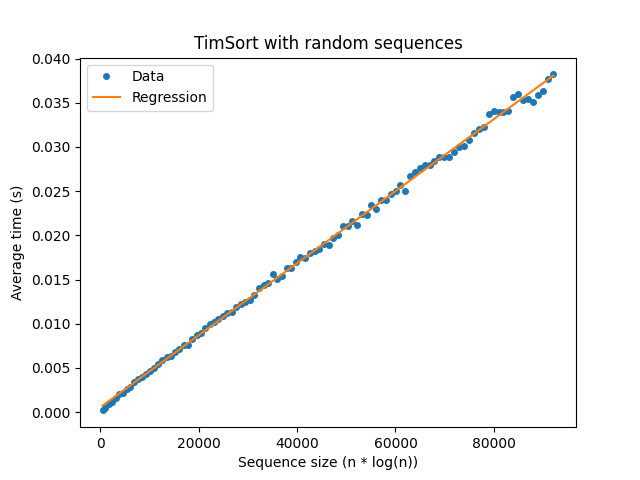
\includegraphics[scale=0.5]{img/plot_random.png}
\vspace{-1em}
\caption{Gráfica con secuencias aleatorias}
\label{fig:grafica:aleatorias}
\end{figure}

La inspección empírica de la gráfica parece revelar que los datos y la regresión siguen la misma tendencia. De la regresión se obtienen los siguientes resultados: \par

\begin{table}[!ht]
\begin{tabular}{|l|r|}
\hline
$a$   & $4.076e-07$ \\ \hline
$b$   & $0.0005474$ \\ \hline
$R^2$ & $0.9987612$ \\ \hline
\end{tabular}
\end{table}

Como se puede evidenciar, el algoritmo obtiene un $R^2 > 0.99$. Esto representa un ajuste bastante alto. Es posible confirmar que, con secuencias aleatorias, este algoritmo tiene una complejidad de $O(n \log n)$.

\subsection{Secuencias ordenadas} \label{resultados:ordenadas}

Para el experimento con secuencias ordenadas, se sigue el protocolo definido en la sección \ref{experimentos:ordenadas}, dando como rango $(b,e,s)$ los datos $(100,10000,100)$. Obtenidos los resultados, se realiza la regresión y se genera el gráfico presentado en la figura \ref{fig:grafica:ordenadas}.

\vspace{-1em}
\begin{figure}[!htb]
\centering
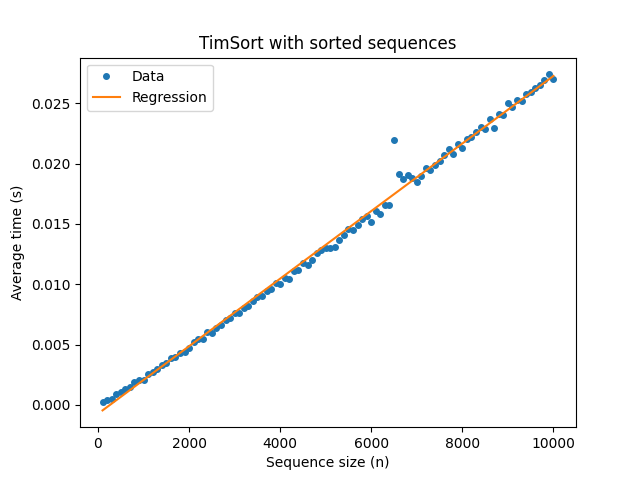
\includegraphics[scale=0.5]{img/plot_sorted.png}
\vspace{-1em}
\caption{Gráfica con secuencias ordenadas}
\label{fig:grafica:ordenadas}
\end{figure}

La inspección empírica de la gráfica parece revelar que los datos y la regresión siguen la misma tendencia. Debido a que los datos ya ordenados es el mejor caso para el algoritmo, la regresión utilizada es una lineal simple de grado 1. Se obtienen los siguientes resultados: \par

\begin{table}[!ht]
\begin{tabular}{|l|r|}
\hline
$a$   & $2.802e-06$ \\ \hline
$b$   & $-0.0007395$ \\ \hline
$R^2$ & $0.9949353$ \\ \hline
\end{tabular}
\end{table}

Como se puede evidenciar, el algoritmo obtiene un $R^2 > 0.99$. Esto representa un ajuste bastante alto. Es posible confirmar que, con secuencias ordenadas, este algoritmo tiene una complejidad de $\Omega (n)$.

\subsection{Secuencias ordenadas invertidas} \label{resultados:invertidas}

Finalmente, para el experimento con secuencias ordenadas invertidas, se sigue el protocolo definido en la sección \ref{experimentos:invertidas}, dando como rango $(b,e,s)$ los datos $(100,10000,100)$. Obtenidos los resultados, se realiza la regresión y se genera el gráfico presentado en la figura \ref{fig:grafica:invertidas}.

\vspace{-1em}
\begin{figure}[!htb]
\centering
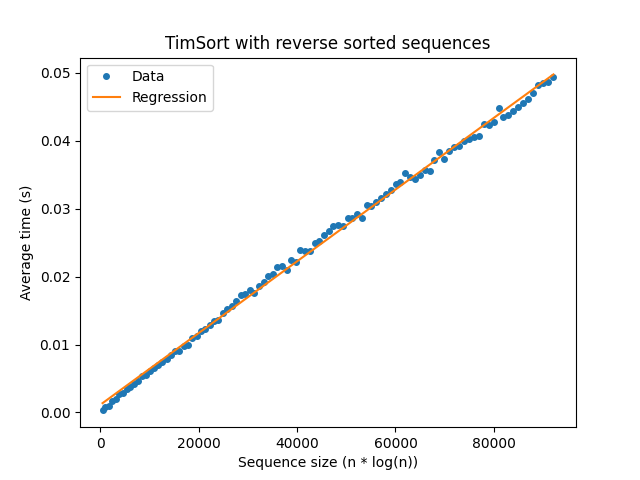
\includegraphics[scale=0.5]{img/plot_reverse_sorted.png}
\vspace{-1em}
\caption{Gráfica con secuencias ordenadas invertidas}
\label{fig:grafica:invertidas}
\end{figure}

La inspección empírica de la gráfica parece revelar que los datos y la regresión siguen la misma tendencia. De la regresión se obtienen los siguientes resultados: \par

\begin{table}[!ht]
\begin{tabular}{|l|r|}
\hline
$a$   & $5.283e-07$ \\ \hline
$b$   & $0.001125$ \\ \hline
$R^2$ & $0.9978855$ \\ \hline
\end{tabular}
\end{table}

Como se puede evidenciar, el algoritmo obtiene un $R^2 > 0.99$. Esto representa un ajuste bastante alto. Es posible confirmar que, con secuencias ordenadas invertidas, este algoritmo tiene una complejidad de $O(n \log n)$.

\end{document}
